\documentclass[12pt]{article}
\usepackage{fullpage,graphicx,psfrag,amsmath,amsfonts,verbatim}
\usepackage[small,bf]{caption}
\usepackage{float}

\input defs.tex

\bibliographystyle{alpha}

\title{Assignment 5 CME 241}
\author{Taylor Howell}

\begin{document}
\maketitle

\newpage
\section*{1. Function Approximation}
For this problem I have implemented methods for function approximation using linear regression (\texttt{linear\_regression.jl}) and neural networks (\texttt{neural\_network.jl}). The results for these implementations are shown in Fig. \ref{linear_regression} and Fig. \ref{neural_network}.
\begin{figure}[!htb]
	\centering
	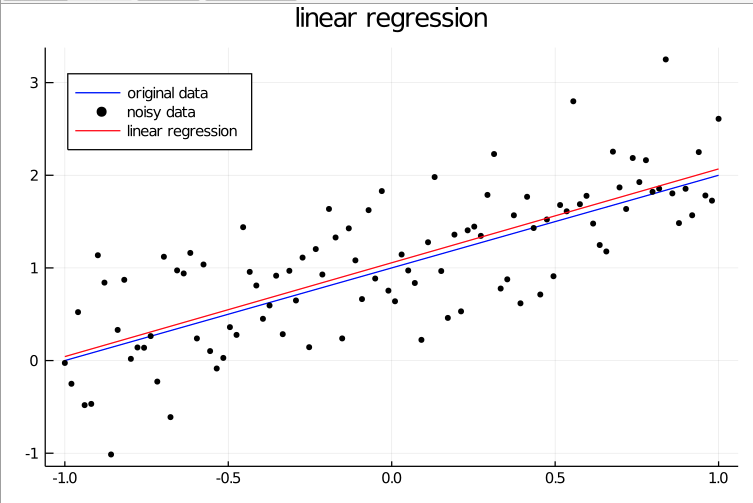
\includegraphics[width=.75\textwidth]{ipad/linear_regression.png}
	\caption{Linear regression. Data is generated with small amounts of Gaussian noise added to a line with slope $m = 1$.}
	\label{linear_regression}
\end{figure}

\begin{figure}[!htb]
	\centering
	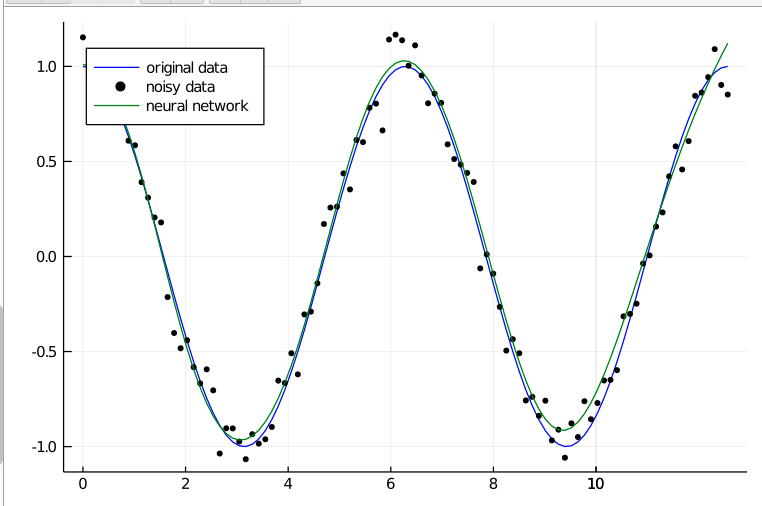
\includegraphics[width=.75\textwidth]{ipad/neural_network.png}
	\caption{Neural-network regression. Data is generated with small amounts of Gaussian noise added to a points from a sinusoidal wave. The network has three layers, with tanh activation functions, and is optimized using Adam with a mean squared error objective function.}
	\label{neural_network}
\end{figure}

\clearpage


\end{document}
